%%%%%%%%%%%%%%%%%%%%%%%%%%%%%%%%%%%%%%%%%%%%%%%%%%%%%%%%%%%%%%%%%%%%%%
%% Technical validation -- standalone working document
%% Paper: Mapping the land-use footprint of Brazilian soy embodied in
%%        international consumption -- a spatially explicit input-output
%%        approach
%%
%% Merge (2026-08-10) of: methods_v2.tex subsec. 2.8 "Validation and
%% uncertainty" (incl. its two figures), the standalone validation.tex
%% (backend consistency, input-assumption sensitivity + table + figure),
%% and the "Uncertainty and sensitivity" subsection of appendix_v2.tex.
%% Self-contained: cross-references into the Methods/Appendix documents
%% are given as plain-text pointers. Compile with:
%%   pdflatex technical_validation && bibtex technical_validation
%%   && pdflatex technical_validation && pdflatex technical_validation
%%%%%%%%%%%%%%%%%%%%%%%%%%%%%%%%%%%%%%%%%%%%%%%%%%%%%%%%%%%%%%%%%%%%%%

\documentclass[pdflatex,sn-nature]{sn-jnl}% Nature Portfolio reference style

\usepackage{graphicx}%
\usepackage{amsmath,amssymb,amsfonts}%
\usepackage{xcolor}%
\usepackage{textcomp}%
\usepackage{manyfoot}%
\usepackage{booktabs}%
\usepackage{geometry}%
\geometry{textheight=240mm}%
\usepackage{float}%
\raggedbottom

\begin{document}

\title[Technical validation]{Technical validation (working document)}

\author*[1]{\fnm{Liza} \sur{Buriak}}\email{TODO@wu.ac.at}

\affil*[1]{\orgdiv{Institute for Ecological Economics},
\orgname{Vienna University of Economics and Business (WU)},
\orgaddress{\city{Vienna}, \country{Austria}}}

\abstract{Standalone draft of the Technical validation section, merging
the Validation and uncertainty subsection of the Methods working
document (methods\_v2), the standalone Validation draft, and the
Uncertainty and sensitivity appendix. The text is self-contained;
pointers to the Methods appendices are given in plain text.}

\maketitle

%%%%%%%%%%%%%%%%%%%%%%%%%%%%%%%%%%%%%%%%%%%%%%%%%%%%%%%%%%%%%%%%%%%%%%
\section{Technical validation}\label{sec:validation}
%%%%%%%%%%%%%%%%%%%%%%%%%%%%%%%%%%%%%%%%%%%%%%%%%%%%%%%%%%%%%%%%%%%%%%

\subsection{Agreement with the Trase benchmark}\label{subsec:val-trase}
The validation targets the subnational half of the pipeline. How much
soy each country imports from Brazil, and how it propagates through
global supply chains to final consumers, is carried by FABIO, a
peer-reviewed global physical input-output database whose construction
and evaluation are documented elsewhere \cite{bruckner2019fabio}; the
pipeline adds no new information at that level. What is new, and
therefore what has to be validated, is the subnational layer: which
municipalities the exported soy comes from and how it is routed to
each importer.

The reconstructed origin-to-importer flows are evaluated against the
independent Trase Brazil--soy dataset (v2.6.1), which links
municipalities of production to countries of first import using
per-shipment customs and logistics records
\cite{godar2015sei,escobar2020trase}. Agreement is measured by the
Pearson correlation between the modelled and the benchmark flows,
computed over all matched municipality--destination pairs of a year
(pooled), for the pairs of one importing country at a time
(per-destination), or on $\log_{10}$ flows in the rocket plots of
Section~\ref{subsec:val-volume}. Two features organise the comparison.
First, agreement depends on flow size: the model and the benchmark
agree closely on the large flows that carry the tonnage and diverge on
the small ones, which are numerous but negligible in volume
(Section~\ref{subsec:val-volume}). Second, from 2019 onward the
comparison target itself changes: Trase switched its per-shipment
source, and part of the post-2018 disagreement originates in the Trase
data rather than in the model (Section~\ref{subsec:val-volume}).

The dependence on volume shapes the choice of the headline metric.
Nearly half of the matched flows (46\%) are below 1{,}000\,t, and
together they carry 1.3\% of the volume (Figure~\ref{fig:rocket}); a
plain average over destinations therefore lets the noise of negligible
flows dominate, giving Cuba the same weight as China. The headline
metric is instead the volume-weighted per-destination correlation: for
each importing country the modelled map of origin municipalities is
correlated with the map Trase reports for that importer, and the
per-importer scores are averaged with the importer's share of the
year's volume as weight (Figure~\ref{fig:weighted}).

\begin{figure}[!tbp]
\centering
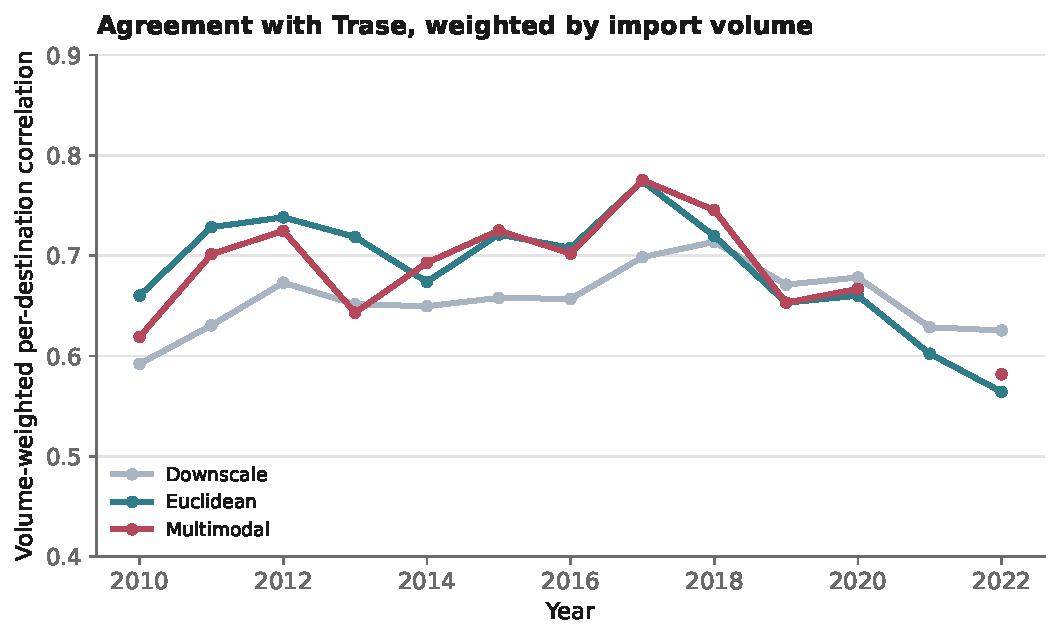
\includegraphics[width=0.78\textwidth]{figures/fig_dest_weighted.pdf}
\caption{Volume-weighted per-destination correlation with the Trase
benchmark, 2010--2022, for the three allocation variants (the
multimodal variant has no 2021 solve). Weights are each importer's
share of the year's Trase-recorded import volume; Brazil (domestic
use) is excluded. The supply-chain models exceed the downscaling
baseline in every year up to 2018; after the benchmark's 2019 change
of source the ordering inverts
(Section~\ref{subsec:val-volume}).}\label{fig:weighted}
\end{figure}

All three allocation variants are compared on this metric: the
downscaling baseline, in which every importer draws from the same
municipal map and only totals differ, the Euclidean model, and the
multimodal transport variant. The weighted correlation of the
Euclidean model runs between 0.66 and 0.77 over 2010--2018 and exceeds
the baseline in every year of that period, by 0.05 to 0.10 in most
years, with the gap closing in 2018; the multimodal variant tracks the
Euclidean model within 0.03 in most years and 0.08 at worst (2013).
Since import totals are
identical in all variants, this gap is exactly the information added
by the supply-chain structure: different importers source from
different parts of Brazil, and only the supply-chain models reproduce
such differences. After 2018 all variants decline and the ordering
inverts, which Section~\ref{subsec:val-volume} traces to the
benchmark's change of source.

The average conceals large differences between destinations. China,
which takes most of the exported tonnage, scores 0.69 to 0.86 across
years and Spain reaches 0.93, while for the smallest importers the
scores scatter widely from year to year, from slightly negative to
above 0.9, with no persistence. The validation appendix of the Methods
document reports the full per-importer trajectories for the four
importers that cover 70\% of the volume and for the five smallest
importers matched in every year.

Part of the distance that remains to the benchmark is a data limitation
rather than a model choice. Installed crushing capacity is published by
ABIOVE as state totals together with a roster of plant locations, with
no capacities for individual plants, so the pipeline has to fix an
allocation rule and divides each state's capacity equally among its
plants; Section~\ref{subsec:val-inputs} quantifies what this assumption
costs. Trase, by contrast, observes individual shipments: per-shipment
customs records name the exporting company, and the company's tax
registration identifies its silos and crushing facilities and their
municipalities, so most of each flow is anchored to a specific
logistics hub before any modelling; only the last step, from the hub to
the municipality of production, is filled by a cost-minimising
allocation similar in spirit to ours \cite{trase2025soymethods}. Per-shipment records of that
granularity are proprietary and not available to an open pipeline.
Sample construction is specified in the validation appendix of the
Methods document.

\subsection{Agreement grows with flow size}\label{subsec:val-volume}
Agreement rises with flow size (Figure~\ref{fig:rocket}). Pooled over
the 91{,}873 matched municipality$\times$destination$\times$year
flows of 2010--2022, which span six orders of magnitude, the correlation of log flows
with Trase is 0.68: large flows converge onto the 1:1 diagonal, small
flows scatter. The same gradient shows in the per-destination scores:
the mean per-destination correlation rises
from 0.29 in the lower half of import volumes to 0.53 in the upper
half.

\begin{figure}[!tbp]
\centering

\includegraphics[width=0.94\textwidth]{figures/rocket_plot_years.pdf}
\caption{Agreement with the benchmark grows with flow size (``rocket
plots''). Every modelled municipality$\times$destination soy export flow is
plotted against the corresponding Trase flow (both $\log_{10}$ tonnes;
flows below 1\,t on either side are excluded) for four sample years.
Because thousands of points overlap, grey contour lines outline where
the point cloud is densest, in the way elevation lines outline a hill;
the dashed line is the 1:1 diagonal on which a perfectly reproduced
flow would lie. Each panel reports the
number of matched flows and the log-scale Pearson correlation. Large
flows converge onto the 1:1
diagonal (the ``nose''), while small flows scatter (the
``plume'').}\label{fig:rocket}
\end{figure}

The weaker agreement visible in the 2020 panel is not specific to that
year but marks the whole 2019--2022 block, and its origin is on the
benchmark side. From 2019 onward Trase switched its per-shipment source
to maritime-only bills of lading that record the country of first
import rather than the final destination, and the share of its exports
with unknown origin municipality roughly doubles
\cite{trase2025soymethods}. At the switch the log-scale correlation
steps down from 0.70--0.74 (2010--2017) to 0.59--0.65 (2019--2022),
and the small flows drift above the diagonal: below 1{,}000\,t the
model reports on average 1.6 times the benchmark value in 2019--2020.
The destination pattern identifies the mechanism. China, served by
direct shipments, is unaffected (mean log deviation 0.00 in 2020),
while Slovenia, whose port of Koper is a transshipment hub for
landlocked Europe, is the strongest outlier in the opposite direction:
the benchmark books to the country of first import the tonnage that
the customs-based model books to final destinations, which in turn
appear mildly over-reported (Thailand, Italy, Germany). Trase itself
recommends against comparing its 2004--2018 and 2019--2022 periods
directly, and the post-2018 part of the correlation band should be
read with that caveat.

\subsection{Sensitivity to input assumptions}\label{subsec:val-inputs}
The sensitivity analysis tests the two input assumptions that the data pin down
least, and where the pipeline therefore has to assume the most:
(a)~the within-state location of crushing: ABIOVE reports capacity
only as state totals, and the baseline divides each state's total
equally among its plants; (b)~the feed and livestock parametrisation:
the GLEAM per-system feed rates and the 2010-frozen municipal herd
composition. Each perturbed variant re-runs the full flow
reconstruction up to the origin-to-importer flows for a representative
year (2019) and is scored against Trase on the pooled
municipality$\times$destination correlation (Euclidean model, base
$r=0.72$); twenty-four variants are run in total. The exact
perturbation recipes are given in the validation appendix of the
Methods document.

For assumption (a), the capacity map is perturbed in three ways:
\begin{enumerate}
\item production-proportional split: each state's capacity is
redistributed across its plant municipalities in proportion to
municipal soybean production (1 run);
\item random splits: individual plant capacities are unobserved, so
every plant is given a positive random weight, drawn from an
exponential distribution, and each state's fixed total is divided
among its plants in proportion to those weights; this makes every
possible split of a state's total equally likely, and repeating it
with ten different random seeds gives ten alternative capacity maps
(10 runs);
\item allocation sharpness: municipal capacities act as weights that
divide the national crush total among municipalities. Under the equal
split they are identical within a state but still differ between
states and where one municipality hosts several plants; raising every
capacity to a power $\gamma$ varies how strongly processing follows
those remaining differences, with $\gamma=2$ concentrating it in the
highest-capacity municipalities and $\gamma=0.5$ spreading it more
evenly (2 runs).
\end{enumerate}

For assumption (b), the parametrisation is perturbed in two ways:
\begin{enumerate}
\item random feed rates: the per-head bean and cake feed rates of every
livestock system are multiplied by random factors, drawn independently
for each system from a lognormal distribution with $\sigma=0.3$, so
that the factors typically lie between 0.75 and 1.35; repeating this
with ten different random seeds gives ten
parametrisations in which the GLEAM rates are wrong by realistic
amounts in different directions (10 runs). The factors average to one
and national feed totals are rescaled to the FAO commodity balance
afterwards, so an error applied uniformly to all systems cancels
exactly; what this perturbation tests is the system mix, since an error
there shifts feed demand toward the municipalities whose herds are rich
in the systems whose feed rates were scaled up in that draw;
\item herd composition: the 2010-frozen municipal herd composition is
replaced by state-average system shares (1 run).
\end{enumerate}

The two assumptions separate cleanly (Table~\ref{tab:val-inputs}).
Crush location accounts for nearly all of the induced variation: the
random within-state splits span correlations of 0.67 to 0.74 (spread
0.073), the production-proportional split scores 0.69, and the
allocation-sharpness variants span 0.024. The feed variants are
immaterial: the ten feed-rate draws move the correlation by less than
0.01 and the herd-composition variant by less than 0.001.

\begin{table}[htbp]
\caption{Input-assumption sensitivity of the model--Trase correlation
(pooled municipality$\times$destination flows, Euclidean model, 2019;
base $r=0.723$).}\label{tab:val-inputs}
\begin{tabular}{@{}llccc@{}}
\toprule
Assumption & Perturbation & Runs & $r$ range & Spread \\
\midrule
Crush location & production-proportional split & 1 & 0.691 & -- \\
Crush location & random within-state splits & 10 & 0.671--0.744 & 0.073 \\
Crush location & allocation sharpness $\gamma\in\{0.5,2\}$ & 2 & 0.706--0.731 & 0.024 \\
Feed rates & random per-system factors (lognormal, $\sigma=0.3$) & 10 & 0.717--0.725 & 0.007 \\
Herd composition & state-average system shares & 1 & 0.722 & -- \\
\botrule
\end{tabular}
\end{table}

\subsection{Backend consistency over time}\label{subsec:val-backend}
Before 2010 the pipeline runs on FABIO v1.1 inputs instead of the v2
build. In the clean overlap years the two backends differ by 6--8\% in
the total footprint with cross-country correlations above 0.988, so
pre-2010 levels are reported unadjusted.

\subsection{Summary}\label{subsec:val-summary}
Taken together, the checks bound the model on every side on which it
can be tested. The reconstructed flows agree with the independent
Trase benchmark at a volume-weighted per-destination correlation of
0.66 to 0.77 over 2010--2018, and the supply-chain structure adds
information exactly where it should, at the destination level, where
it exceeds a structure-free baseline in every year of that period.
Agreement is strongest where the tonnage is: the flows that carry the
footprint are the best-validated part of the distribution, with China
scoring 0.69 to 0.86 across years. The reconstruction is
stable under perturbation of its weakest inputs: across twenty-four
perturbed re-runs the benchmark correlation stays between 0.67 and
0.74 around a base of 0.72, the feed and herd assumptions are
immaterial, and the residual
sensitivity is concentrated in a single known data gap, the
within-state location of crushing capacity, which per-plant capacity
data would close. The remaining modelling choices are equally bounded:
the multimodal transport variant performs on par with the
straight-line model, and the FABIO backend vintage shifts pre-2010
levels by 6--8\% while leaving the cross-country pattern intact.
Results for large flows and large importers can therefore be used with
confidence, while results for individual small-volume destinations
should be read with the caution that Section~\ref{subsec:val-volume}
quantifies.

\bibliography{refs}%

\end{document}
